% ------------------------------------------------------------------------
%	Compile in draft mode to get response to the reviewers
% ------------------------------------------------------------------------
% isresponse can be passed on the command line
% pdflatex "\def\isresponse{1} \input{foo.tex}"

\def\isresponse{1}

\ifdefined\isresponse
  \documentclass[12pt, draft]{article}
\else
  \documentclass[12pt]{article}
\fi

% For selectively turning things on and off in the draft
\usepackage{ifdraft}

% Spacing, math, code listing, color, crossrefs in pdf
\usepackage[margin=1in]{geometry} % 1in margin all around
\usepackage{setspace, amsmath, listings, xcolor}
\usepackage[hyphens]{url}
% Graphics. Always show the figures but float to the end
\usepackage[final]{graphicx, subfig}
\usepackage{endfloat}
% Improve the line breaking to reduce the number of overfull boxes
\usepackage[final]{microtype}

% Citations are numbers, with round parenthesis
% no brackets around numbers in the bibliography
% use the CBE/CSE bib style
\usepackage[numbers,round]{natbib}
\renewcommand{\bibnumfmt}[1]{#1.}
\bibliographystyle{mrm}

% Equations have square brackets around them
\makeatletter
  \def\tagform@#1{\maketag@@@{[#1]\@@italiccorr}}
\makeatother

% Spacing and indentation
\setlength{\parindent}{0pt} % No paragraph indent.
\setlength{\parsep}{12pt}   % Paragraph separation.
\setlength{\parskip}{12pt}  % Paragraph skip.

% For notes and reviewer responses and crossrefs to them and stuff
% Always use the hyperref package in final mode
\usepackage[final]{hyperref}
\ifdefined\isresponse
	\hypersetup{colorlinks=true}
	\usepackage[draft]{changes}
\else
	\hypersetup{colorlinks=false}
	\usepackage[final]{changes}
\fi

% This makes clickable references to the reviewer questions
\makeatletter
\def\namedlabel#1#2{\begingroup#2\def\@currentlabel{#2}\phantomsection\label{#1}\endgroup}

% This defines a question as an item (enumerated list) with label
\newcommand{\question}[1]{\item[\namedlabel{q#1}{#1}]}
% Color the responses
\newcommand{\response}[1]{\textcolor{cyan}{#1}}
% Put the question reference in the margin
\setremarkmarkup{\marginpar{\ref{q#2}}}
% Reduce typing
\newcommand{\madded}[2][None]{\added[remark=#1]{#2}}
\newcommand{\mreplaced}[2][None]{\replaced[remark=#1]{#2}}
\newcommand{\mdeleted}[2][None]{\deleted[remark=#1]{#2}}

% ------------------------------------------------------------------------
%	Manuscript specific bits
% ------------------------------------------------------------------------
% Set the graphics path
\graphicspath{{./figures/}}

% Include the git sha-1 hash of the repo
\IfFileExists{githash.txt}
{\newcommand{\githash}{\input{githash.txt}}}
{\newcommand{\githash}{(NONE)}}

% ------------------------------------------------------------------------
%	Document start
% ------------------------------------------------------------------------
\begin{document}

% ------------------------------------------------------------------------
%	Response to Referees
% ------------------------------------------------------------------------
\ifdraft{

\section*{Referee 1 Comments and Responses}
\subsection*{Summary}
In this work, the authors propose a standardized, vendor-agnostic file format for storing the raw data collected by MRI scanners, with the goal of increasing the reusability of developed computational tools and facilitating reproducible research. Whereas other medical imaging disciplines developed such frameworks many years ago (e.g., DICOM, NIfTI, etc...), MRI is lacking in this area and would greatly benefit from such development. Personally, I am strongly in favor of the efforts that have been put forth by the authors and commend their efforts here and in leading to this stage. I also understand that the role of this manuscript is two-fold: 1) a description of the current state of the project; and 2) and advertisement for involvement from the MRI community. Therefore, it is somewhat different than your standard research article. Overall, the manuscript is well-written and logically ordered. However, at the same time, I felt that a number of important aspects of the standard were either insufficiently or too vaguely discussed, which left me (as someone already aware of and in favor of this project) with some hesitations/aversions. Additionally, I also felt that the paper and its impact would greatly benefit from the inclusion of some more advanced examples. However, with appropriate revisions, I believe this paper will be become a very important part of the MRI literature.

\begin{itemize}
\question{R1.1} One significantly absent part of this paper is a definition of what is ``raw'' data. To different people even within the MRI community, this can mean very different things. To me, raw data is MRI data that has been completely untouched by any processing whatsoever. This means no gridding/ramp sampling correction, coil compression/combination, zero padding, parallel imaging reconstruction, partial Fourier, etc..... To others, something like post-GRAPPA, post-Homodyne k-space data that hasn't yet been zero-padded and DICOM-encoded might be ``raw''. Back when the ISMRM Fat+Water toolbox came out, this issue came up because some of the ``raw'' complex image data had actually been coil combined ? some people thought this was a non-issue while others were unhappy about the pre-processing. Given the tag ``raw data format'', I think there needs to be a very clear specification of what is and isn't raw data, and a more clear discussion about how these distinctions will be made.

\response{We agree with the reviewer completely with the reviewer as to the definition of ``raw data".  We have added some text in various parts of the text and we have hopefully clarify and reinforced the point that raw data means completely untouched by any processing - as close as possible to the output of the analog to digital converters.}

\question{R1.2} In effort to promote the flexibility of the ISMRM XML+HDF5 file format structure, the authors have painted a picture of almost too much flexibility ? which raises the question of how is any type of real ``standardization'' going to be maintained? Are there any elements in the header that must always be present and defined in an ISMRMRD file, e.g., data dimensions? In other words, what exactly is guaranteed to be common amongst every single ISMRMRD file? This should be presented very explicitly.

\response{The reviewer is correct in pointing out that we have emphasized the flexibility provided by the file format and have somewhat downplayed issues  related to ``standardization".  We believe at this early stage it is difficult to foresee the ways in which different practitioners will chose to use the format for their specific applications, and more importantly, the challenge is not technical, but rather sociological.  A consensus needs to emerge around the description of a particular type of experiment, where the community agrees on the meaning of various parameters stored in the XML header and individual acquisition headers.  We do believe however that the file format itself does provide a great deal of structure and provides a framework within which these discussions can take place.  We have added text to the ``Design" section discussing this point.  We have also added a description of the requirement that the file format specify a clear set of rules for data organization (the schema and data structures) and have added a description of the minimal dataset: the ISMRMRD XML header is required to contain 1 instance of the experimentalConditions type and 1 instance of the encoding type.  The addition of the spiral and EPI examples should also help to clarify the flexiblity/structure tradeoff.}

\question{R1.3} Many types of MRI reconstruction problems require multiple data sets of different types, such as parallel imaging as mentioned. It's discussed that the file format can incorporate both raw data and some image data, such as coil sensitivity profiles, but it was unclear to me whether several different raw data sets can be packaged into one file? For example, suppose I am doing a SENSE recon and have both k-space data for both my cal scan and accelerated acquisition. However, I am interested in experimenting with different coil profile estimation algorithms ? can I store both raw data sets in one file, since they go together?

\response{Yes, multiple data sets can be stored in the same ISMRMRD file.  We have added text and a more complex example with a noise scan, a gradient echo sequence to measure coil sensitivity maps, and data from an accelerated EPI sequence to highlight this feature.}

\question{R1.4} Are there any limits on the dimensionality of the raw data?

\response{The maximum number of acquisitions per data set is $2^32 - 1 \approx 4\times10^6$ acquisitions because the scan\_counter is stored as a 32 bit unsigned integer.  This should be sufficient for current scanner technology.  Each acquisition can contain $2^16 - 1 = 65535$ samples because the number\_of\_samples is stored as a 16 bit unsigned integer.  Both of these could be increased up to 64bits.  The HDF5 file format has a 64bit limit on the number of elements in a dataset (acquisitions in this case).}

\question{R1.5} One issue that is not discussed is vendor proprietary information. Most vendors typically do not make readily available publically their raw data file structure without first entering into some type of research agreement. It seems as though the availability of file ?conversion? tools would require you to establish and maintain some type of agreement with all of the vendors. This process, including what has been established so far and what still needs to be done, should be elaborated on. I also noted that the provided link for the GE conversion tool is not yet publically available ? is this at all related to such research agreements?

\response{The GE converter repository is private only because it includes some source code (header files) from the GE pulse programming environment.  If someone wished to have a publicly released GE converter, then this bit of code, which is required to read the GE raw files, would need to be replaced with code free of any GE encumbrances.  The Siemens, Philips, and Bruker converters are released without approval from the respective vendors, and no such approval is required. The converters contain no proprietary code and the parts of the code that interact with the vendor raw data file, parse header and data structures etc, can be reverse engineered in a tedious but straightforward manner.  It is helpful, but not necessary to maintain research agreements with any/all of the vendors.}

\question{R1.6} As vendors release new system software versions, etc..., who will be maintaining and updating the conversion tools and ensuring their correctness?

\response{As vendors release new software versions, the members of the research community who are users of that platform will need to contribute their expertise to update the conversion tools and to ensure their correctness. The process under which this necessary work will be carried out is as yet undetermined, and one can imagine various ways in which it could be accomplished. Presumably, there would be some sort of board or governing committee drawn from the members of the ISMRM.  No matter which structure is decided upon, it is our belief that this work is best done by those that have a vested interest in it, and that in general, it is usually preferable to keep formalized processes and rules to a minimum. We have added some text to the discussion regarding this point.}

\question{R1.7} This manuscript would greatly benefit from including more, and more complex, usage examples beyond the basic case in Fig. 3. Please add some additional examples demonstrating what the general file structure would be for some cases where different and multiple types of raw data are needed. Some examples that would be useful that come immediately to mind to me are: 1) a multi-channel spiral scan with a dual-echo cal (raw) data set for B0 map estimation; 2) a SENSE type parallel imaging scan with both a body and phased array cal scan; 3) a multi-shot, ramp-sampled EPI scan with zero and first order eddy current phase data; and 4) a randomly sampled acquisition like commonly used in compressed sensing applications.

\response{We have added two more complex examples.  The first is a spiral sequence with a nominal k-space trajectory and a gradient impulse response function corrected trajectory stored for every acquisition.  The second is an accelerated EPI sequence with several calibration scans.  These two examples provide the reader with a sense of what is possible with the flexibility that is provided by the format.}

\end{itemize}

\section*{Referee 2 Comments and Responses}
\subsection*{Summary:}
This paper seeks to be the official/citable introduction of the open source raw data format proposed by the International Society for Magnetic Resonance in Medicine (ISMRM) known as the ISMRMRD format. The ISMRMRD format originates from a subcommittee formed at the 2013 ISMRM Sedona, Arizona workshop on image reconstruction. The authors present a strong case about the need for a vendor-neutral (non-proprietary) file format for MR research and development, especially in light of the widespread push for reproducible research across all disciplines of biomedical science. The manuscript also describes the design strategy, general specifications and some implementation details of the file format. An extremely important development since the establishment of the ISMRMRD itself is a set of mostly open-source converters to transform vendor-specific raw data files from Bruker, GE, Philips or Siemens to ISMRMRD. As evidence of the capabilities of ISMRMD and the associated converters, image reconstructions of a phantom object (kiwi fruit) are presented using data acquired on Bruker, GE, Philips and Siemens scanners. Reconstructions are shown using application programming interfaces (APIs) based on MATLAB, Python and C++. The authors provide all raw data and reconstruction code freely on-line.

This paper has high potential to be an important contribution to the MRI research community, however, there are many concerns (mostly minor) that need to be addressed before acceptance for publication. Because this paper will likely be the first introduction to the ISMRMRD format for many MRI researchers, it needs to attract support and avoid leaving open questions that may turn away potential users. If the ISMRMRD format is not widely adopted, it will fail. This paper can either make or break the case for adoption. The concerns of this reviewer are outlined below as general and specific comments.

\subsection*{General Comments:}
\begin{itemize}
\question{R2.1} The most important addition to the paper, which I require in order to support acceptance for publication, is a table clearly showing the ISMRMRD encoding counters as rows (\texttt{kspace\_encoding\_step\_1}, \texttt{kspace\_encoding\_step\_2}, average, slice, contrast, phase, repetition, set, segment, user) and how the data dimensions of the considered vendors (Bruker, GE, Philips and Siemens) map into those encoding dimensions. For example it is not at all clear how commonly encountered data dimensions such as diffusion encoding direction, diffusion b-value, arterial spin labeling on/off, etc. map into the established ISMRMRD encoding counters. If a converter for a given vendor in its current form does not handle a certain common dimensionality, e.g. DWI/DTI, it should be noted. Nothing will turn off potential users faster than the disappointment of the converters not being able to handle very common scan types.

\response{We have added a section describing the encoding counters and flags and have included a table showing the relationship between the ISMRMRD counters and the counters for the four vendors.  We now discuss more explicitly the current lack of a well articulated convention for many specific applications and use DWI and ASL as two examples of the lack of formal application specific guidelines.}

\question{R2.2} Related to the above, the existence and intended use for the \texttt{user\_int} and \texttt{user\_float} arrays in the acquisition header and the user array in the encoding counters is not addressed anywhere in the text. Please add to the text a description of the envisioned purpose for these arrays. Their existence provides flexibility, but it also creates the potential for incompatibility if users and developers harness the user defined arrays differently.

\response{As the reviewer correctly points out, these arrays are included to provide flexibility and unfortunately also create the potential for incompatibility.  We have added a paragraph to the ``Design'' section discussing the need for flexibility and highlighting the potential for incompatibility.}

\question{R2.3} I am particularly concerned about the omission of a third \texttt{kspace\_encode\_step}, which leaves out easy support for 3D spectroscopic imaging. Please address this omission in the text and discuss how to support 3D spectroscopy with ISMRMRD.

\response{Unfortunately \texttt{kspace\_encode\_step\_0} was omitted from the encoding counters in version 1 of the C-structs. (Although it is included in the encoding limits in the XML schema.)  We thank the reviewer for pointing out this oversight.  An issue (\#42) has been opened on GitHub and the oversight will be corrected in version 2 of the format.  We have added a sentence to the text in order to describe this issue.}

\question{R2.4} Is spectroscopy otherwise fully compatible with ISMRMRD? In either case, please add statements about the compatibility with spectroscopy to the manuscript.

\response{As far as we know the ISMRMRD format is fully compatible with spectroscopy (except for the caveat discussed in the previous question.)  Unfortunately none of the authors of the manuscript are particularly attuned to the needs of the spectroscopy community and there will certainly be experiments that are currently difficult to describe in the current format.  Of course we welcome any and all input from the members of the MR community who are interested in this application.  We have added a few sentences discussing spectroscopy support.}

\question{R2.5} More needs to be said about how the community will work together in the future to make changes to the ISMRMRD format. For example, will everything be driven from the GitHub repositories? Will there be future ISMRM committees formed? What about a standing committee? Ultimately, who specifically has commit authority on the official GitHub repositories and how will that person or person(s) be selected in the future?

\response{Michael, this one is yours.}

\question{R2.6} Related to the above, there are already some choices in the fixed acquisition and encoding header that may not be adequate in the future. The use of uint16 (65,536 values) to represent \texttt{measurement\_uid} and kspace encoding steps may already be inadequate to handle sequences that exist today. Many fMRI and DTI scans existing today already produce nearly 20,000 images from single-shot EPI readouts, which would each require a unique \texttt{measurement\_uid}. What happens when uint16 is not enough?

\response{An earlier version of the format used uint16 to store the measurement\_uid. The current version of the format uses uint32. The typographical error and has been corrected. Note that the measurement\_uid is meant to encode a unique ID for the measurement (series) and the scan\_counter is meant to store the acquisition number within a given measurement. The scan\_counter is also stored as a nint32 which should be sufficient for current scanner technology, although it could be increased in a future version to uint64 which is currently the limit in HDF5 for the number of elements in a dataset.   Note: latex the markup tool cannot be used in figures.}

\question{R2.7} The role of the flags in the acquisition header is not mentioned anywhere, and there are many, many flags defined for ISMRMRD. Please add something about the flags if only to state the role, a few examples, and where to go to learn more.

\response{A mention of the flags and a brief description of their use has been added in the section with responses for R2.1 and R2.2.}

\question{R2.8} The manuscript states that the GE converter is private and only available within the GE MRI research converter. Does this mean that Bruker, Philips and Siemens granted permission to make their converters open source?

\response{The GE converter is private only because it includes some source code from the GE pulse programming environment.  If someone wished to have a publicly released GE converter, then this bit of code, which is required to read the GE raw files, would need to be replaced with code free of any GE encumbrances.  The Siemens, Philips, and Bruker converters are released without approval from the respective vendors, and no such approval is required. The converters contain no proprietary code and the parts of the code that interact with the vendor raw data file, parse header and data structures etc, can be reverse engineered in a tedious but straightforward manner.}

\question{R2.9} Related to the above, please state in the manuscript what type of software license ISMRMRD and the open-source converters are distributed under. Two of the open-source converters (Bruker and Philips) appear to not have a LICENSE file.

\response{All of the software released by this project is developed in part by an employee of the US Federal government in the course of his official duties.  It is released into the public domain and pursuant to title 17 section 105 of the United States Code is not subject to copyright protection.  Thank you for pointing out the lack of LICENSE files for the Bruker and Philips converters.  This oversight has been corrected.}

\question{R2.10} Many potential users of the domain-specific ISMRMRD format may be skeptical of the underlying domain-independent HDF5 format. I strongly suggest spending more time discussing how HDF5 comes from the National Center for Supercomputing Applications (NCSA). Also, please give more citations/examples of how HDF5 is being use in biomedical science, e.g., the Biological Observation Matrix (BIOM) format described at http://www.biom-format.org. Other on-going and completed projects involving HDF5 are listed at http://www.hdfgroup.org/projects

\response{We have added several sentences to the ``File container" section addressing this point.  We thank the reviewer for suggesting the references to BIOM and the list projects involving HDF5.}

\question{R2.11} I strongly suggest adding a description of a known gotcha with the HDF5 format. HDF5 files include creation dates for the file and objects within a file. Actually multiple dates are supported (creation, last access, modification). This typically causes HDF5 files containing the exact same data to have different checksum values. To accurately compare two HDF5 files, a utility such as h5diff should be used. In fact, the paper should mention the existence (and download location) of hdf5 utilities and hdf5 viewers.

\response{We have added a few sentences just after the additions for the previous question pointing the reader to the hdf5 utilities and viewers and mentioning the issue with needing hf5 specific tools for diff.}

\question{R2.12} I confirmed that the image repository is downloadable, but I suggest posting the data using the EU-supported zenodo.org that will also create digital object identifiers (DOIs) for the data set that are easily citable. In fact, zenodo.org can also easily create DOIs for a specific release of the cited GitHub repositories.

\response{We thank the reviewer for the excellent suggestion.  We have posted a copy of the data to zenodo and have hooked to the GitHub repositories to generate DOIs for each release.  The DOIs for the releases specific to this manuscript have been added to the text.  We have discontinued the use of XNAT as we have found it difficult to use for this type of data.}

\question{R2.13} Not all dependencies for ISMRMRD and the converters are mentioned/cited such as FFTW, boost libraries, libXML, and libXSLT. Please add them to the text.

\response{The currently implementation of the ISMRMRD C++ API for creating and reading from and writing to files only depends on HDF5 at runtime and CMake and HDF5 at build time.  The xmlheader handling depends on pugixml which is distributed with the source code.  The utilities for generated a test phantom and the simple reconstruct program depend on FFTW and boost.  The converters depend on ISMRMRD, Boost, libXML and libXST.  We have added some clarification in the text.}

\question{R2.14} ``Matlab'' is used several places instead of ``MATLAB''. Please use ``MATLAB'' consistently.

\response{MATLAB is now capitalized throughout.}

\question{R2.15} Throughout the paper, the word ``handcrafted'' is used. Please replace with ``custom'' or ``customized'' as appropriate.

\response{The term ``handcrafted'' is well known in the computing literature. A Google search for ``handcrafted software'' returns approximately 1~million hits.  It serves to indicate custom code that is written by a human programmer, e.g. the C++ XML Header interface class, as opposed to custom code that is machine generated, e.g. the Python XML Header interface class which is generated by processing the XML schema file with the PyXB program.}

\end{itemize}

\subsection*{Specific Comments}
\begin{itemize}
\question{R2.16} Page 5: 4th bullet point: Please state that arrays are indexed from zero, and that is how 0 to 11 with center at index position 5 describes 12 ky values -5 (index 0) to +6 (index 11).

\response{Done}

\question{R2.17} Page 5: 4th bullet point: How would ky lines that are symmetrically spaced about DC be represented? In other words, lines that have a 0.5 delta\_k shift from those described in bullet point 4.

\response{The current implementation of cartesian encoding is not able to handle this particular use case.  An acquisition collected with even sampling in kx at non-integer ky could be described as a non-cartesian trajectory.  The traj field could be used to indicate that ky is constant for the acquisition with a value of 4.5 (say).}

\question{R2.18} Page 6: ISMRMD Library: Line 1: Please add ``domain-independent'' before Hierarchical Data Format.

\response{Done}

\question{R2.19} Page 6: File container: Line 5: Please add that HDF5 is used for MATLAB's .mat format starting with mat-file version 7.3 (MATLAB R2006b or later).

\response{Done}

\question{R2.20} Page 8: 3rd bullet: Please provide a citation/URL for CMake

\response{Done}

\question{R2.21} Page 11: Item 3: Please change ``Real (experimental)'' to ``Experimental''

\response{Done}

\question{R2.22} Page 11: Item 5: Please change ``synthetic and real'' to ``synthetic and experimental''

\response{Done}

\question{R2.23} Page 11: Item 6: Please clarify ``put into production in a clinical environment'' with ``given approval from a local ethics board''. Certainly, you do not want to give readers the impression that ISMRMRD is automatically sanctioned/approved for clinical use.

\response{Done}

\question{R2.24} Page 12: Please specify that the noise level for the shepp logan phantom was 0.05 (the default value of the utility). Also, is that 0.05 value a noise sigma (or noise variance, sigma squared) on a normalized 0.0 to 1.0 scale?

\response{0.05 is the standard deviation of the noise added to the real and imaginary part of each receiver channel.  It is in absolute units.  The signal level depends on the phantom parameters and the coil receive profiles, therefore it is difficult to report the exact SNR of the measurement in a straightforward fashion as the noise in the reconstructed image is spatially varying, etc.  A small phrase has been added to hopefully clarify the description of the noise amplitude.}

\question{R2.25} Page 12: last line: ``The resulting are shown'' should be something like ``The resulting reconstructions are shown''

\response{Done}

\question{R2.26} Page 14: Line 3: Please add that ``wget'' is needed for the \texttt{do\_get\_data.sh} script and that the script is intended for Linux/Apple.

\response{As suggested in one of the questions above, we have chosen to use zenodo to distribute the data files - this provides a nice URL that can be used from a browser.  The description of the procedure for getting the data has been modified to reflect this change.  A comment has been added to clarify that the optional script is intended to be used on Linux/Apple.  The script has also been modified to use curl (installed by default on both Linux and Apple).}

\question{R2.27} Page 15: Line 8: HDF5 is inherently compressed already, right? Is this referring to a different kind of compression?

\response{The reference was to vendor file formats that are support compression, not ISMRMRD. HDF5 supports various forms of compression but none are enabled by default, and we have not yet explored what would be most appropriate for MR data.  A clarification phrase has been added.}

\question{R2.28} Figure 2: Can a 3D kspace trajectory with kx, ky, kz coordinates be stored as well?

\response{Yes, storage of 3D space trajectories with kx, ky, kz coordinates is fully supported.  The phrase ``k-space sampling locations" in the caption refers to this capability.  It has been changed to ``k-spacing trajectory sampling locations".  Note: latex the markup tool cannot be used in figure captions.}

\question{R2.29} Figure 4: The 32-ch GE and 32-ch Siemens results look shaded compared to the Bruker and Philips images. Bruker was a single-channel coil, but Philips was a 6-channel coil. Is the shading caused by the GE and Siemens being in a larger head coil while the Philips data was acquired in a smaller knee coil? The shading should be mentioned/addressed in the text or else some readers may incorrectly assume there is a problem with the conversion/reconstruction.

\response{Correct, this is due to the respective receiver array inhomogeneity. A clarification sentence has been added. Note: the latex markup tool cannot be used in figure captions.}

\end{itemize}

% Print out the list of modifications
\listofchanges

}% end of \ifdraft

% ------------------------------------------------------------------------
%	Full Title Page
% ------------------------------------------------------------------------
\newpage
\clearpage
\pagestyle{empty}

\begin{center}
\large \textbf{ISMRM Raw Data Format: A Proposed Standard for MRI Raw Datasets}

\normalsize
\singlespacing
Souheil~J.~Inati$^1$,
Joseph~D.~Naegele$^1$, 
Nicholas~R.~Zwart$^2$,
Vinai~Roopchansingh$^1$,
Martin~J.~Lizak$^3$,
David~C.~Hansen$^4$,
Chia-Ying~Liu$^5$,
David~Atkinson$^6$,
Peter~Kellman$^7$,
Sebastian~Kozerke$^9$,
Hui~Xue$^7$,
\madded[R1.7]{Adrienne~E.~Campbell-Washburn$^7$},
Thomas~S.~S{\o}rensen$^8$,
Michael~S.~Hansen$^7$
\end{center}

\begin{flushleft}
\begin{enumerate}
\item National Institute of Mental Health, National Institutes of Health, Bethesda,~MD
\item Keller Center for Imaging Innovation, Barrow Neurological Institute, Phoenix,~AZ
\item National Institute of Neurologic Disease and Stroke, National Institutes of Health, Bethesda,~MD
\item Department of Oncology, Aarhus University Hospital, Aarhus, Denmark
\item Radiology and Imaging Sciences, Clinical Center, National Institutes of Health, Bethesda,~MD
\item Centre for Medical Image Computing, University College London, United Kingdom
\item National Heart, Lung, and Blood Institute, National Institutes of Health, Bethesda,~MD
\item Department of Clinical Medicine, Aarhus University, Aarhus, Denmark
\item Institute for Biomedical Engineering, University and ETH Zurich, Zurich, Switzerland
\end{enumerate}
\end{flushleft}

%\vspace{2mm}
Correspondence to: \\
Michael S. Hansen \\
National Heart, Lung, and Blood Institute, NIH \\
NIH Building 10/B1D405 \\
10 Center Drive \\
Bethesda, MD 20892 \\
\textit{michael.hansen@nih.gov} \\

\textit{Running Head:  ISMRMRD}

%\vspace{2mm}

\textit{Submitted to Magnetic Resonance in Medicine} 

%\vspace{2mm}

\textit{Word count: 3904} % reported by texcount (total-abstract-top)

% ------------------------------------------------------------------------
%	Abstract
% ------------------------------------------------------------------------
\newpage
\clearpage
\pagenumbering{arabic} % begin numbering here
\pagestyle{plain}
\doublespacing
\section*{Abstract}
\textbf{Purpose:}  This work proposes the ISMRM Raw Data (ISMRMRD) format as a common MR raw data format, which promotes algorithm and data sharing.\\
\textbf{Methods:} A file format consisting of a flexible header and tagged frames of k-space data was designed. Application Programming Interfaces were implemented in C/C++, MATLAB, and Python. Converters for Bruker, General Electric, Philips, and Siemens proprietary file formats were implemented in C++. Raw data were collected using MRI scanners from four vendors, converted to ISMRMRD format, and reconstructed using software implemented in three programming languages (C++, MATLAB, Python).\\
\textbf{Results:} Images were obtained by reconstructing the raw data from all vendors. The source code, raw data, and images comprising this work are shared online, serving as an example of an image reconstruction project following a paradigm of reproducible research.\\
\textbf{Conclusion:} The proposed raw data format solves a practical problem for the MRI community.  It may serve as a foundation for reproducible research and collaborations.  The ISMRMRD format is a completely open and community-driven format, and the scientific community is invited (including commercial vendors) to participate either as users or developers.

\textit{Abstract word count: 197} % reported by texcount (abstract)

% ------------------------------------------------------------------------
%	Keywords
% ------------------------------------------------------------------------
\textbf{Keywords:}  MRI, Image reconstruction, Open source, Raw data format

% ------------------------------------------------------------------------
%	Body
% ------------------------------------------------------------------------
\newpage
\clearpage
\onecolumn

% ------------------------------------------------------------------------
%	Introduction
% ------------------------------------------------------------------------
\section*{Introduction}
Image reconstruction research has played a pivotal role in driving many advances in magnetic resonance imaging. Examples of paradigm shifting techniques include parallel imaging~\cite{Pruessmann:1999uq, Sodickson:1997fk, Griswold:2002kx}  and, more recently, the introduction of nonlinear reconstruction and compressed sensing~\cite{Donoho:2006compressed, Lustig:2007vn}. Novel reconstruction algorithms build on and improve existing methodology, and most reconstruction articles compare new methods to existing methods in terms of image quality and reconstruction speed.

Reproducible research has drawn a great deal of attention recently, as highlighted for example in a recent special issue of Science~\cite{Jasny:2011again, Peng:2011reproducible}. The field of computational science in particular has produced several excellent examples of how such research can be carried out, e.g., the wavelab toolbox~\cite{wavelab}.  The ISMRM has begun to take steps to help facilitate reproducible research, e.g., with the MRI unbound website~\cite{mri_unbound}. Underlying many of these efforts is a discipline-specific file format specification that allows scientists to exchange data easily.  Much of modern astronomy research, for example, relies on telescope data in the FITS standard~\cite{fits}.  Other discipline-specific data formats have enabled scientists to escape from the limitations imposed by vendor-specific, proprietary technology, leading to the development of a wide range of post-acquisition data analysis tools, and enabling large-scale collaborations.  Medical imaging has the DICOM standard~\cite{dicom}, which allows radiology departments to store data from different vendors on a centralized PACS, and computer scientists to implement novel image processing methods in a vendor neutral manner. The subfield of neuroimaging has NIfTI~\cite{nifti}, which underlies large-scale projects like the human connectome project~\cite{connectome}. The image file formats are useful for disciplines that operate on the reconstructed images, but they do not address the needs of scientists involved in the development of image reconstruction algorithms. This paper proposes an MR-specific raw data format. 

This ISMRMRD standard was developed by a subcommittee of the ISMRM Sedona 2013 workshop.  It is designed to capture the details of the MRI experiment in a way that permits image reconstruction.  It is important to note that this goal is fundamentally different from that of proprietary vendor raw data file formats.  Generally, proprietary vendor raw file formats are intended to capture protocol parameters for a particular pulse sequence at the time of the scan.  The proprietary raw data file formats are intended to store the information needed to reproduce a particular experiment on a specific version of the scanner software and reconstruction framework.  The tight coupling between 1) the scanner console user interface, 2) the pulse sequence control parameters, and 3) the image reconstruction control parameters, make the vendor formats depend on a great deal of proprietary, vendor-specific knowledge. The quantity of hidden information makes these formats inconvenient for data sharing.  More importantly, the specific implementation details of a particular vendor's scanner software architecture greatly influences the design of these file formats and the type of information that they contain.  In contrast, the proposed standard is designed to facilitate the exchange of the raw k-space data along with the physics parameters of the data acquisition process to provide the information necessary for image reconstruction.

While the ISMRMRD format will continue to evolve as it attracts more users with a more diverse set of applications and needs, the basic format has remained stable for more than two years, and it makes sense to present it to the MRI community. This paper lays out the design and structure of the format and describes several software tools that have been developed to interact with data in the proposed format. A number of vendor-specific tools have been created for converting proprietary data formats to the proposed format. An overview of the current status of these data converters and information needed to locate them is also provided. As a demonstration of how the data format can be used, a phantom has been scanned on four different scanners, the data converted to ISMRMRD and reconstructed with several different open source reconstruction programs written in  \mreplaced[R2.14]{MATLAB}{Matlab} (The MathWorks), Python, and C++ programming languages. 

All software, data, figures, scripts to generate the figures, and the text in this manuscript are available as open source. 

% ------------------------------------------------------------------------
%	Methods
% ------------------------------------------------------------------------
\section*{Methods}
\subsection*{Design}
The proposed ISMRMRD format combines a flexible header (XML-based) with fixed structures for the data. These are packaged together into a single file.  A minimal raw data set is depicted in Fig.~\ref{fig:format} and consists of two sections:
\begin{itemize}
\item{XML header.} A flexible XML format document that can contain an arbitrary number of fields and accommodate everything from simple values (matrix sizes, etc.) to entire vendor protocols, etc. The purpose of this XML document is to provide parameters that may be meaningful for some experiments but not for others. This XML format is defined by an XML Schema Definition file (\texttt{ismrmrd.xsd}).
\item{Raw data.} This section contains all the acquired data in the experiment organized as a sequence of data items.  Each data item corresponds to a single data frame or chunk in an experiment, for example, a single line of data in a Cartesian acquisition or a single interleave in a multi-shot spiral acquisition. Each data item consists of a fixed-size header (C-struct) with encoding numbers, etc., along with the k-space data for all of the acquired channels, and (optionally) the k-space trajectory as depicted in Fig.~\ref{fig:cstruct}. The raw data structures are defined in a C/C++ header file (\texttt{ismrmrd.h}).
\end{itemize}
The proposed format also provides a simple image format for storing the product of reconstructions and a multidimensional array format for storing additional user-specified parameters (e.g., gradient nonlinearity correction maps, etc.).

% Figure 1
\begin{figure}
\begin{center}
\includegraphics[width=6in]{figure1_ismrmrd_format.eps}
\caption{A minimal ISMRMRD dataset consists of a flexible XML header and raw data organized as sequence of data items consisting of fixed-size data headers and the corresponding k-space data for each set of samples or data chunk.}
\label{fig:format}
\end{center}
\end{figure}

\subsubsection*{Encoding counters, flags}
R2.1 table for counters comparison to vendors
     diffusion encoding direction, diffusion b-value, arterial spin labeling on/off, etc. map into the established ISMRMRD encoding counters
     \madded[]{Fig.~\ref{fig:cstruct}}

R2.2 User int


% Figure 2
\begin{figure}
\begin{center}
\includegraphics[width=6in]{figure2_uml_diagram.eps}
\caption{The raw data structure for each data frame or chunk of the acquisition, consisting of a fixed-size header with encoding numbers, location, etc. and the raw k-space data and (optionally) the k-space trajectory sampling locations. \textbf{r} and \textbf{i} indicate the real and imaginary part of the data points respectively.}
\label{fig:cstruct}
\end{center}
\end{figure}

\subsubsection*{Encoding Space}
One of the key design features of the proposed format is the notion of an ``encoding space", which is a description of the type and limits of the experiment and provides the reconstruction program with the physical size and resolution of the imaging volume and the ranges of the data header labels.  An ISMRMRD dataset may contain data from several encoding spaces.  Each encoding space is described in the XML header, and each acquisition (data chunk) is tagged with a label for the encoding space from which it was acquired. All encoding spaces have a trajectory type, an ``encodedSpace," a ``reconSpace", ``encodingLimits", and an optional trajectory description, that can contain an arbitrary set of named parameters such as the gradient ramp and flat top times for EPI, or the parameters controlling the shape of the spiral trajectory, etc.  An example of an encoding describing a simple 2D Cartesian acquisition is shown in Fig.~\ref{fig:encoding}.  In this particular case, the encoding has the following description:
\begin{itemize}
\item the ``encodedSpace" section gives the matrix size ($32\times16\times1$) and field of view in mm ($600\times300\times10$) of the imaging volume encoded by the excitation, i.e.,  a 10~mm thick slice, 600~mm in x and 300~mm in y, encoded with a nominal matrix size of 32 in x and 16 in y, i.e., at a nominal resolution of 18.75mm.
\item The ``reconSpace" section indicates that the image should be reconstructed on a smaller field of view ($300\times300\times10$), but with half the number of pixels in x.
\item The combination of the ``encodedSpace" and ``reconSpace" indicates that the \mreplaced[]{$k$}{k}-space data were acquired on a grid oversampled by a factor of 2 in the x direction.
\item The ``encodingLimits" section indicates \mreplaced[R2.16]{the ky center (5) and the minimum and maximum ky values (0 and 11 respectively)}{the bounding box of the sampled region of $k$-space using arrays that are indexed from zero, therefore in this case the 12 points with indices from $0$ to $11$ with center at index $5$ indicate the 12 $ky$ points from $-5$ (index 0) to $+6$ (index 11) with center at $ky=0$ (index 5)}, i.e., this is a partial Fourier experiment, with a true pixel size that is somewhat larger than the nominal resolution\mdeleted[R2.16]{, $min(ky)=-5$, $max(ky)=+6$}.
\end{itemize}

% Figure 3
\begin{figure}
\begin{center}
\includegraphics[width=6in]{figure3_encoding_spaces.eps}
\caption{The encoding space of a simple 2D Cartesian acquisition.  The XML header describes the image encoding and reconstruction fields of view and matrix sizes and k-space sampling bounding box.  The image is acquired at a matrix size of 32 $\times$ 16 $\times$ 1 and field of view of 600mm $\times$ 300mm with a slice thickness of 10mm.  It should be reconstructed at a matrix size of 16 $\times$ 16 $\times$ 1 and field of view of 300mm $\times$ 300mm with a slice thickness of 10mm.   The k-space data were acquired on a grid oversampled by a factor of 2 in the x direction.  The ``encodingLimits" section indicates the ky center (5) and the minimum and maximum ky values (0 and 11 respectively), i.e. this is a partial Fourier experiment, with a true pixel size that is somewhat larger than the nominal resolution, $min(ky)=-5$, $max(ky)=+6$. The example experiment also employs partial Fourier along the readout dimension, i.e. asymmetric echo.}
\label{fig:encoding}
\end{center}
\end{figure}

\subsubsection*{Application specificity}
R2.2 User int, float
R2.4 - Spectroscopy

\subsection*{ISMRMRD Library}
The ISMRMRD library is a cross-platform implementation based on the \madded[R2.18]{domain-independent} Hierarchical Data Format (HDF) (\url{http://www.hdfgroup.org/HDF5}) for storage and provides C/C++, Python, and MATLAB (Mathworks) interfaces for reading and writing ISMRMRD files.  The project follows an open source development model with a website at (\url{http://ismrmrd.github.io}) and a discussion board and code repositories at \url{http://github.com/ismrmrd}.  The library and associated tools can be compiled in a straightforward way on Linux, Windows, and Apple computers.  This section provides a high-level description of the implementation and discuss some of the choices made during the development process.  The reader is encouraged to examine and experiment with the source code for more a detailed view.

\subsubsection*{File container}
The HDF format was chosen as the binary file container.  The HDF format is very flexible and has been adopted broadly in the scientific community.  Reading and writing from the HDF format are supported by most programming languages and computational environments.  The HDF library has a core C and C++ API, is supported natively in MATLAB (it forms the basis for MATLAB's own ``.mat" file format \madded[R2.17]{starting with mat-file version 7.3 (MATLAB R2006b) or later}), and is supported in Python via the H5Py package (\url{http://www.h5py.org}).

\subsubsection*{XML header data binding}
The XML header can be thought of as a text representation of relevant experimental parameters that are needed for meaningful image reconstruction. When writing image reconstruction software, the software developer usually interacts with a binary representation of the XML document (XML Data Binding) to avoid direct, error prone, and tedious interaction with the XML text. The process of generating the binary representation of the XML document (deserialization) and the generation of the XML document from the binary representation (serialization) is handled by dedicated functions. Both the binary representation and the functions for serialization and deserialization can be auto-generated by XML data binding tools, e.g., CodeSynthesis XSD (\url{http://www.codesynthesis.com/products/xsd/}) for C++, JAXB for Java (\url{https://jaxb.java.net/}), or PyXB (\url{http://pyxb.sourceforge.net/}) for Python. The auto-generated data structures and functions are easier to maintain since they can be regenerated when the XML schema (\texttt{ismrmrd.xsd}) changes, but the syntax they provide can be less convenient. Alternatively, data structures and serialization and deserialization code can be "handcrafted". This may provide a more convenient interface, but the software maintenance overhead is greater. The proposed data format does not dictate which approach to use when interacting with the XML header, but the provided libraries include data structures and associated functions. Depending on the convenience of available tools these software components have either been "handcrafted" or auto-generated as described below.  

\subsubsection*{Programming language-specific implementations}
This work is implemented in three different programming environments or languages to interact with ISMRMRD files. This section contains a few notes regarding the C/C++, MATLAB, and Python APIs that were created:
\begin{itemize}
\item{C library.}  This code defines fixed data structures (\texttt{ismrmrd.h}) and the functions used to interact with the HDF5 file.
\item{C++ library.} This code is a wrapper around the C library with classes and functions that provide memory management and reduce programming error.  It includes a ``handcrafted'' XML header binding class.  
\item{Build system.} The C and C++ implementation use the CMake (Kitware\madded[R2.20]{, \url{https://cmake.org}}) build configuration system to support multiple operating systems (Linux, Microsoft Windows, Apple OS X).
\item{MATLAB library.} This code consists of pure MATLAB data structures and functions (classes) that call the MATLAB interface to HDF5 as well as ``handcrafted'' Java code for the XML header binding class using the Java provided by MATLAB.
\item{Python library.} This code consists of pure Python classes for the data structures, uses NumPy arrays for the data and the k-space trajectories (\url{http://www.numpy.org}), and an auto-generated XML header binding class.
\end{itemize}

The code repositories also contain the source code for the documentation (which use the Doxygen (\url{http://www.doxygen.org}) and Sphinx (\url{http://sphinx-doc.org}) projects) as well as \mreplaced[R2.13]{example utility programs demonstrating}{examples of} how to use the APIs to read and write ISMRMRD files.  \madded[R2.13]{The utility programs depend on the Boost library (\url{http://boost.org}) for command-line user interaction.}

\subsection*{Data Conversion Tools}
Converters have been developed for several proprietary file formats: Bruker, General Electric, Philips, and Siemens.  The Bruker, Philips and Siemens converters are open source with repositories that can also be found at \url{http://github.com/ismrmrd}.  The GE converter relies on proprietary vendor code and is being distributed via the vendor's research network.  Given the variety in vendor raw data file formats, the architecture of these programs is described in general terms with the aim of giving some guidance or aid to others who are implementing their own conversion tools.  The reader is referred to the source code for  details, but to give a few examples: the Bruker raw data are stored in a simple directory structure with the acquisition parameters stored in several text files and k-space data stored in a simple binary file as equal length frames of k-space data; there are no data labels associated with each data frame. Siemens raw data are stored in a single integrated file that can contain raw data from multiple scans.  For each scan, acquisition parameters are stored in a structured text header, followed by k-space data frames stored in acquisition order, where each frame of k-space data is tagged with data labels containing the frame's line number, slice number, location, etc. The complexity of the GE and Philips formats fall somewhere between the simple file structure of the Bruker format and the more integrated file format used on the Siemens systems. The GE data does not contain explicit labels for each data frame and more sequence knowledge is needed to convert the data. The Philips raw data format has data labels associated with each data frame and it was possible to design a more generic automated converter. 

The converters for the aforementioned vendor formats were written in C++. \madded[R2.13]{All four converters use the CMake build system and depend on the ISMRMRD C/C++ library described above as well as Boost for user interaction.  For XML file handling, the converters also depend on  either 1) libXML2 and libXSLT (\url{http://www.xmlsoft.org}) on Linux and Apple, or 2) the Xerces-C XML parser library (\url{http://xerces.apache.org/xerces-c/}) on Windows.}  Acquisition parameters from the vendor-specific data were converted to an intermediate XML file (containing vendor-specific parameter names and values). This  XML file was then translated into the vendor-independent ISMRMRD XML header file using a sequence-specific Extensible Stylesheet Language (XSL) style sheet. The frames of k-space data were processed in the order in which they appeared on disk.  For formats with tagged data frames (Philips and Siemens), the proprietary binary header tags were parsed and used to populate the fixed-size ISMRMRD data header structures.  For formats with untagged data frames (Bruker and GE), sequence and vendor-specific knowledge was used.  

It is worth emphasizing that creating the converters required significant work and special knowledge of the vendor formats. However, once code was developed for converting raw data from one pulse sequence on a particular platform, it was straightforward to modify this code to handle other sequences. It is expected that other developers can modify these converters to handle currently unsupported product sequences or their own research sequences. It is also important to note that while some users may work on the implementation of these vendor-specific converters, many users will simply use the converted ISMRMRD files as input for the algorithms and thus be exposed less to these vendor-specific details as a consequence of using the proposed format. 

\subsection*{Experimental Demonstrations}
In a typical MR image reconstruction research project, one often tests and validates an algorithm or a particular implementation of an algorithm. This validation can be done using simulated data and data acquired from phantom or in vivo experiments.  In the interest of reproducible research, a scientist could distribute the source code and the raw data sets that were used to generate the figures for the publication and perhaps additional code or data related to the testing or validation of the algorithm.

This section demonstrates how one could use the ISMRMRD format and APIs for the development, implementation, and testing of an image reconstruction algorithm suitable for 2D experiments.

\subsubsection*{Example 1: Cross-vendor and cross-language demonstration}
In this example, the k-space data are acquired using a multi-channel receiver array and the data are fully sampled on a Cartesian grid.  The workflow for this demonstration project could form a subset of a full development cycle:
\begin{enumerate}
\item An initial implementation or proof of concept of the algorithm is implemented in a rapid prototyping language such as \mreplaced[R2.14]{MATLAB}{Matlab} or Python.
\item Synthetic data are generated in simulation and used to test/validate the prototype implementation.
\item \mreplaced[R2.21]{Experimental}{Real (experimental)} data are collected and used to test/validate the prototype implementation.
\item A high performance production version of the algorithm is implemented in a compiled language such as C/C++ or Fortran.  In some cases the high performance implementation may require specialized hardware such as a compute cluster or a graphical processing unit (GPU).
\item The synthetic and \mreplaced[R2.22]{experimental}{real} data sets are used to test/validate the high performance implementation of the algorithm.
\item The high-performance implementation of the algorithm is \madded[R2.23]{given approval from a local ethics board and} put into production in a clinical environment.
\end{enumerate}

The prototype image research example project began with an outline of the steps of the simple 2D image reconstruction algorithm:
\begin{enumerate}
\item Data are read and stored in a buffer (Nkx,Nky,Ncoil).
\item The Fourier transform is computed in two dimensions (x,y).
\item The images are cropped if the data were acquired on an oversampled grid in the frequency encode direction.
\end{enumerate}
The prototype implementation of this algorithm was written in Python (\texttt{do\_recon\_python.py}) and \mreplaced[R2.14]{MATLAB}{Matlab} (\texttt{do\_recon\_matlab.m}).  The high-performance implementation of the algorithm was written in C++ (\texttt{ismrmrd\_recon\_cartesian\_2d}).  All three implementations used the corresponding ISMRMRD APIs to read in an ISMRMRD format file and to save the reconstructed image.

A synthetic data set in ISMRMRD format was generated using a program written in C++ (\texttt{ismrmrd\_generate\_cartesian\_shepp\_logan}).  This program simulated a simple experiment collecting data from a single-slice object using an 8-element receive array in the presence of a small amount of noise.  The k-space data were generated by multiplying the Shepp-Logan phantom with the receive profile of an 8-rung birdcage coil followed by Fourier transformation and the addition of randomly generated white Gaussian noise \madded[R2.24]{with standard deviation 0.05 to the real and imaginary part of each receiver channel}.

Data sets were collected from a phantom (kiwi fruit) using scanners from four different vendors: 
\begin{itemize}
\item Bruker 4.7T with a single channel 10cm transmit/receive coil
\item GE 3T MR750 with a 32-channel head coil
\item Philips Achieva 3T with a 6-channel knee coil
\item Siemens 3T Skyra with a 32-channel head coil
\end{itemize}
Data were acquired using product 2D pulse sequences.  The FOV=10~cm, slice thickness=2~mm, and matrix size (Nx=Ny=512) were matched, although no attempt was made to match the pulse sequence type or timings.

\subsubsection*{Example 2: Non-cartesian trajectories, nominal vs. corrected}
\madded[R]{
A spiral imaging data set is used to illustrate the optional k-space trajectory data included in the ISMRMRD format. Imaging data was acquired on a 1.5T Siemens system (32 spiral interleaves, FOV = 30 cm, slice thickness = 5cm, matrix size = 192). True k-space trajectories were predicted using the gradient impulse response function~\cite{Vannesjo2013, Campbell-Washburn2015} and stored with the k-space data in the ISMRMRD format.  A reconstruction program was written in MATLAB (\texttt{do\_spiral\_recon\_matlab.m}) to generate images using the ISMRMRD trajectory data and nominal variable density spiral trajectories.  
}

\subsubsection*{Example 3: Accelerated EPI with GRE coil sensitivity calibration and SENSE reconstruction}
\madded[R2]{
Multiple data sets.
}

\section*{Results}

\subsection*{Experimental Demonstration}
The raw data files were transferred off-line and converted into ISMRMRD using the vendor-specific converters described above. It was possible to convert the data from all four vendors. The resulting \madded[R2.25]{reconstructions} are shown in Fig.~\ref{fig:demo}.

% Figure 4
\begin{figure}
\begin{center}
\includegraphics[width=6in]{figure4_recon_demo.eps}
\end{center}
\caption{An experimental demonstration where data sets were acquired on scanners from four vendors and converted from the vendor proprietary raw data file formats into ISMRMRD format.  A fifth data set was synthesized numerically and stored in ISMRMD format.  The five ISMRMRD raw data sets were reconstructed using three image reconstruction programs written in C++, MATLAB, and Python.  The resulting images are shown above, from left to right Bruker, General Electric, Philips, Siemens, and the synthetic data set,  and from top to bottom C++, MATLAB, and Python reconstruction programs. The differences in SNR and shading between the images are due to the coil geometries: small volume coil vs. knee coil vs. head array.}
\label{fig:demo}
\end{figure}

\madded[R2]{
Figure~\ref{fig:spiral} shows spiral images reconstructed using the ISMRMRD trajectories and nominal variable density spiral trajectories. The trajectory data stored in the ISMRMRD format incorporates contemporary system-specific calibration data to produce distortion corrected images during real-time or retrospective reconstruction.
}
% Figure 5
\begin{figure}
\begin{center}
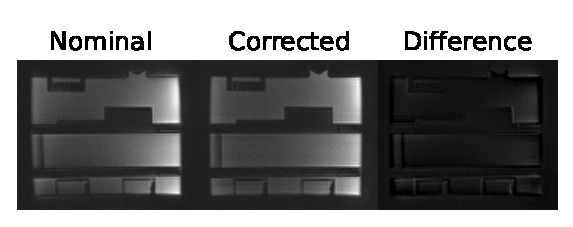
\includegraphics[width=6in]{figure5_spiral_demo.eps}
\end{center}
\caption{Images reconstructed with nominal variable density spiral trajectories compared to spiral trajectories stored in ISMRMRD format. ISMRMRD trajectories are predicted using contemporary gradient impulse response functions and therefore produce distortion-corrected reconstructed images. }
\label{fig:spiral}
\end{figure}

\subsection*{Source Code and Raw Data Dissemination}
The source code for this project is being distributed in several git repositories hosted on GitHub at the URLs listed bellow.  The SHA-1 hashes uniquely identify the particular revision of each of the repositories used for the production of this manuscript:
\begin{itemize}
\item Manuscript LaTeX, figures and \mreplaced[R2.14]{MATLAB}{Matlab} and Python reconstruction: \\
	\url{https://github.com/ismrmrd/ismrmrd-paper} \\
	hash=\githash
\item C++ API and C++ synthetic data generation and C++ reconstruction: \\
	\url{https://github.com/ismrmrd/ismrmrd} \\
    	hash=e7ecb1bbc93c62aceaeb8d197016d67b44e07fee
\item Python API: \\
	\url{https://github.com/ismrmrd/ismrmrd-python} \\
	hash=4e2d8be17ad14fc9ff8d5801751a4511ce435b39
\item Bruker converter: \\
	\url{https://github.com/ismrmrd/bruker_to_ismrmrd}\\
	hash=46dbb5720e9f4304af0920cd6dfa5f7370c75d89
\item GE converter (currently private):\\
	 \url{https://github.com/nih-fmrif/ge-tools} \\
	 hash=f63f74e61e2f8bc920164aa5c8e6ef4dd22705b0
\item Siemens converter:\\
	 \url{http://github.com/ismrmrd/siemens_to_ismrmrd}\\
	 hash=a740086b831c5b259aca36a41a3654b04c672b03
\item Philips converter: \\
	\url{https://github.com/ismrmrd/philips_to_ismrmrd}\\
	hash=b5256ed8267446e70059a5eea88ae6de59c12fe7
\end{itemize}
The raw data in vendor proprietary formats and in ISMRMRD format are being distributed via GitHub (\url{https://github.com/ismrmrd/ismrmrd/releases/download/v1.2.3-data/ismrmrd_data.zip})\mdeleted[R2.26]{XNAT (http://central.xnat.org) under the project ``ISMRMRD Paper" with ID ``ISMRMRD"}.  Alternatively the raw data can be downloaded using the \texttt{code/do\_get\_data.sh} script \madded[R2.26]{which is intended for Linux/Apple}. Readers are encouraged to download the data and source code.

% ------------------------------------------------------------------------
%	Discussion
% ------------------------------------------------------------------------
\section*{Discussion and Conclusion}
This work presents an initial version of a standard for storing raw MR data and an implementation that supports several common programming languages and operating systems. It has also been demonstrated that data can be converted to ISMRMRD from proprietary vendor formats. Once the data have been converted to a vendor-independent format, generic reconstruction tools can be used to reconstruct data regardless of the scanner origin. The presented data converters are not complete for all proprietary configurations. However, the data converters are either completely available as open source or shared freely in the research communities associated with a specific vendor platform. Following the approach laid out in the source code for the data conversion software it should be a relatively simple task to accommodate other acquisition types. 

The methods presented in this paper focused on a 2D Cartesian reconstruction example for simplicity, but more sophisticated reconstruction systems also use the ISMRMRD format. For example, the Gadgetron \cite{Hansen:2013aa} framework uses the format as its internal data representation. The Graphical Programming Interface \cite{Zwart:2014aa} has also been used with the ISMRMRD format using a set of externally provided compute nodes (\url{https://github.com/hansenms/gpi_ismrmrd}).

Future work will be focused on expanding the header sections in the flexible XML header to support specific applications. Changes to the fixed memory layout (C-struct) header and data may include capabilities to store arbitrary waveform data elements that could be used to capture detailed information about gradient waveforms or physiological telemetry. The format may also be changed to allow more choices for data storage formats and precision. Specifically, data is currently stored as 32-bit floating point values, which causes ISMRMRD files to be larger than the original data from vendors that use fixed point (integer) storage either in 16-bit format or in combination with variable length integer encoding (compression). The proposed format is flexible enough to accommodate different storage forms, possibly in combination with compression, \madded[R2.27]{which is easily supported by HDF5}, but support for such features is not currently included in the software libraries.  

The main aim of the proposed standard is that it will serve as a foundation upon which practitioners can base reproducible research and collaborations.  A great deal of work remains and the authors ask for input from the ISMRM community to help shape the direction of the format. Specifically, the project would benefit from volunteers that have a detailed understanding of more specialized research applications in terms of which experimental parameters are needed to produce high quality reconstructions. The authors would also like to encourage groups with existing software packages to adopt this open data format as one of the input formats they support. 

It is important to reiterate that the ISMRMRD format is a completely open and community-driven format. The authors and developers invite anybody in the community (including commercial vendors) to participate either as users of the format or as developers of the format or associated tools.

% ------------------------------------------------------------------------
%	Acknowledgments
% ------------------------------------------------------------------------
\section*{Acknowledgements}
Multiple people participated in the discussions that led to this work.  The authors acknowledge their contributions (in no particular order): 
Walter F. Block,
Peter Boernert,
David O. Brunner,
Mark A. Griswold,
Brian A. Hargreaves,
Craig H. Meyer,
Sonia Nielles-Vallespin,
Tim Nielsen, 
Douglas C. Noll,
James G. Pipe,
Kaveh Vahedipour, and
Ghislain Valliant.

This research was supported in part by the Intramural Research Program of the NIH, NHLBI, NIHM, NINDS.

% ------------------------------------------------------------------------
%    References
% ------------------------------------------------------------------------
\bibliography{ismrmrd}




\end{document}
